% Created by tikzDevice version 0.7.0 on 2015-01-10 18:42:07
% !TEX encoding = UTF-8 Unicode
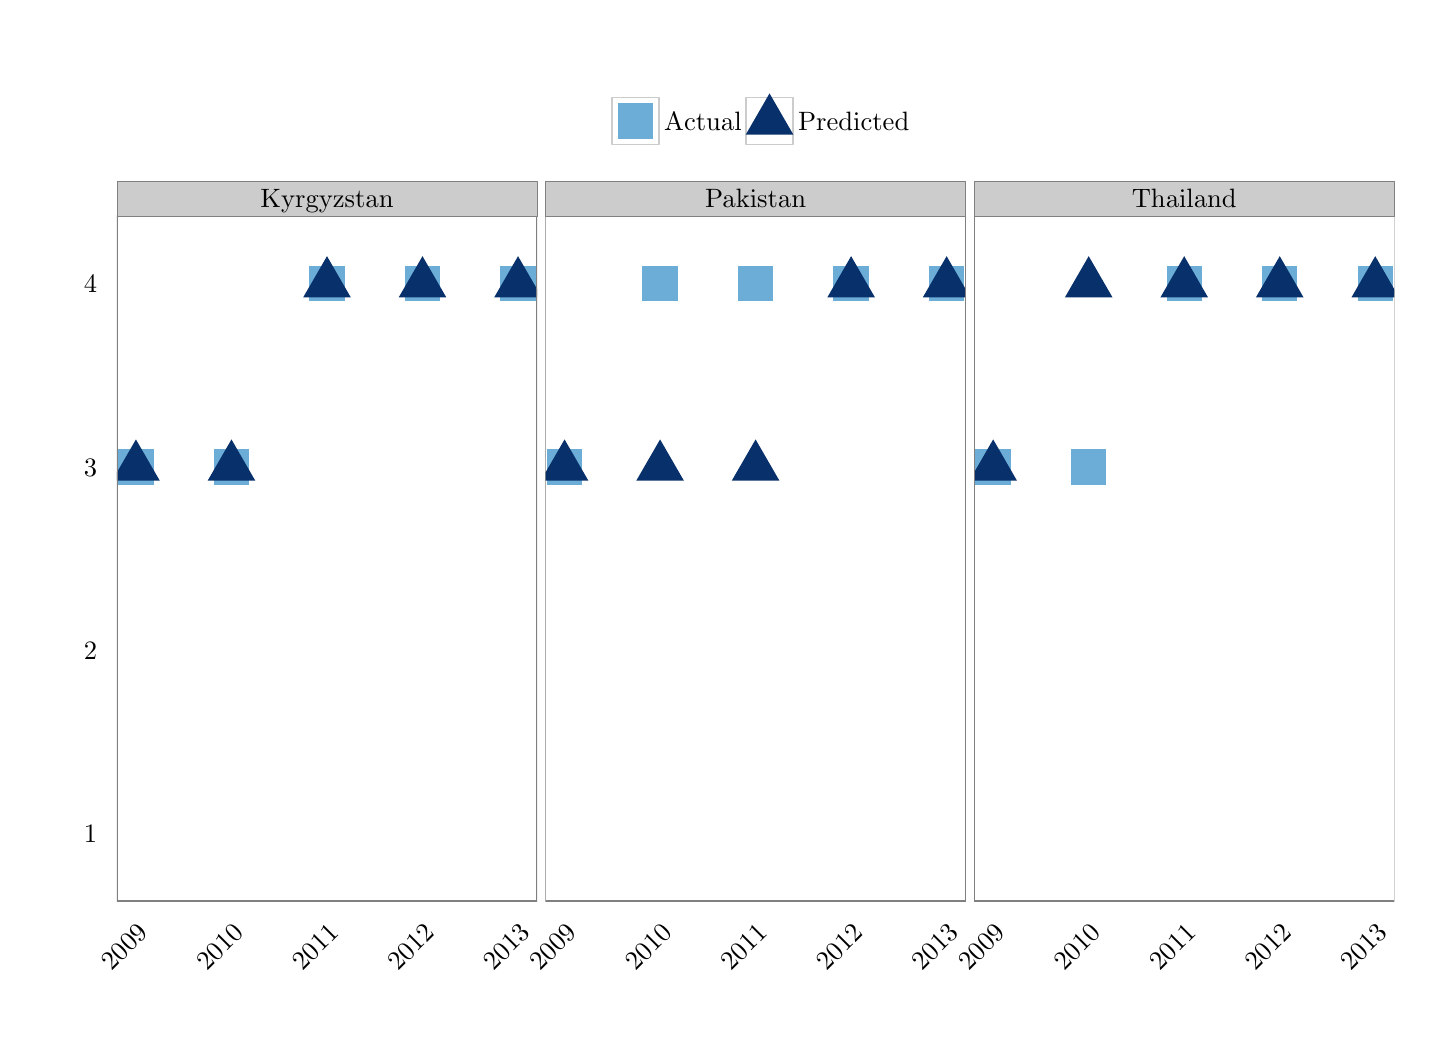
\begin{tikzpicture}[x=1pt,y=1pt]
\definecolor[named]{fillColor}{rgb}{1.00,1.00,1.00}
\path[use as bounding box,fill=fillColor,fill opacity=0.00] (0,0) rectangle (505.89,361.35);
\begin{scope}
\path[clip] (  0.00,  0.00) rectangle (505.89,361.35);
\definecolor[named]{drawColor}{rgb}{1.00,1.00,1.00}
\definecolor[named]{fillColor}{rgb}{1.00,1.00,1.00}

\path[draw=drawColor,line width= 0.6pt,line join=round,line cap=round,fill=fillColor] ( -0.00,  0.00) rectangle (505.89,361.35);
\end{scope}
\begin{scope}
\path[clip] ( 32.22, 45.67) rectangle (184.09,293.33);
\definecolor[named]{fillColor}{rgb}{1.00,1.00,1.00}

\path[fill=fillColor] ( 32.22, 45.67) rectangle (184.09,293.33);
\definecolor[named]{fillColor}{rgb}{0.42,0.68,0.84}

\path[fill=fillColor] (101.75,262.43) --
	(114.56,262.43) --
	(114.56,275.23) --
	(101.75,275.23) --
	cycle;

\path[fill=fillColor] ( 67.24,196.21) --
	( 80.04,196.21) --
	( 80.04,209.01) --
	( 67.24,209.01) --
	cycle;

\path[fill=fillColor] (170.78,262.43) --
	(183.59,262.43) --
	(183.59,275.23) --
	(170.78,275.23) --
	cycle;

\path[fill=fillColor] (136.27,262.43) --
	(149.07,262.43) --
	(149.07,275.23) --
	(136.27,275.23) --
	cycle;

\path[fill=fillColor] ( 32.72,196.21) --
	( 45.53,196.21) --
	( 45.53,209.01) --
	( 32.72,209.01) --
	cycle;
\definecolor[named]{fillColor}{rgb}{0.03,0.19,0.42}

\path[fill=fillColor] (108.16,278.78) --
	(116.78,263.85) --
	( 99.53,263.85) --
	cycle;

\path[fill=fillColor] ( 73.64,212.56) --
	( 82.26,197.63) --
	( 65.02,197.63) --
	cycle;

\path[fill=fillColor] (177.19,278.78) --
	(185.81,263.85) --
	(168.56,263.85) --
	cycle;

\path[fill=fillColor] (142.67,278.78) --
	(151.29,263.85) --
	(134.05,263.85) --
	cycle;

\path[fill=fillColor] ( 39.12,212.56) --
	( 47.75,197.63) --
	( 30.50,197.63) --
	cycle;
\definecolor[named]{drawColor}{rgb}{0.50,0.50,0.50}

\path[draw=drawColor,line width= 0.6pt,line join=round,line cap=round] ( 32.22, 45.67) rectangle (184.09,293.33);
\end{scope}
\begin{scope}
\path[clip] (187.10, 45.67) rectangle (338.97,293.33);
\definecolor[named]{fillColor}{rgb}{1.00,1.00,1.00}

\path[fill=fillColor] (187.10, 45.67) rectangle (338.97,293.33);
\definecolor[named]{fillColor}{rgb}{0.42,0.68,0.84}

\path[fill=fillColor] (256.63,262.43) --
	(269.44,262.43) --
	(269.44,275.23) --
	(256.63,275.23) --
	cycle;

\path[fill=fillColor] (187.60,196.21) --
	(200.40,196.21) --
	(200.40,209.01) --
	(187.60,209.01) --
	cycle;

\path[fill=fillColor] (222.12,262.43) --
	(234.92,262.43) --
	(234.92,275.23) --
	(222.12,275.23) --
	cycle;

\path[fill=fillColor] (291.15,262.43) --
	(303.95,262.43) --
	(303.95,275.23) --
	(291.15,275.23) --
	cycle;

\path[fill=fillColor] (325.66,262.43) --
	(338.47,262.43) --
	(338.47,275.23) --
	(325.66,275.23) --
	cycle;
\definecolor[named]{fillColor}{rgb}{0.03,0.19,0.42}

\path[fill=fillColor] (263.03,212.56) --
	(271.66,197.63) --
	(254.41,197.63) --
	cycle;

\path[fill=fillColor] (194.00,212.56) --
	(202.62,197.63) --
	(185.38,197.63) --
	cycle;

\path[fill=fillColor] (228.52,212.56) --
	(237.14,197.63) --
	(219.90,197.63) --
	cycle;

\path[fill=fillColor] (297.55,278.78) --
	(306.17,263.85) --
	(288.93,263.85) --
	cycle;

\path[fill=fillColor] (332.06,278.78) --
	(340.69,263.85) --
	(323.44,263.85) --
	cycle;
\definecolor[named]{drawColor}{rgb}{0.50,0.50,0.50}

\path[draw=drawColor,line width= 0.6pt,line join=round,line cap=round] (187.10, 45.67) rectangle (338.97,293.33);
\end{scope}
\begin{scope}
\path[clip] (341.98, 45.67) rectangle (493.85,293.33);
\definecolor[named]{fillColor}{rgb}{1.00,1.00,1.00}

\path[fill=fillColor] (341.98, 45.67) rectangle (493.85,293.33);
\definecolor[named]{fillColor}{rgb}{0.42,0.68,0.84}

\path[fill=fillColor] (376.99,196.21) --
	(389.80,196.21) --
	(389.80,209.01) --
	(376.99,209.01) --
	cycle;

\path[fill=fillColor] (411.51,262.43) --
	(424.31,262.43) --
	(424.31,275.23) --
	(411.51,275.23) --
	cycle;

\path[fill=fillColor] (446.02,262.43) --
	(458.83,262.43) --
	(458.83,275.23) --
	(446.02,275.23) --
	cycle;

\path[fill=fillColor] (480.54,262.43) --
	(493.34,262.43) --
	(493.34,275.23) --
	(480.54,275.23) --
	cycle;

\path[fill=fillColor] (342.48,196.21) --
	(355.28,196.21) --
	(355.28,209.01) --
	(342.48,209.01) --
	cycle;
\definecolor[named]{fillColor}{rgb}{0.03,0.19,0.42}

\path[fill=fillColor] (383.40,278.78) --
	(392.02,263.85) --
	(374.77,263.85) --
	cycle;

\path[fill=fillColor] (417.91,278.78) --
	(426.53,263.85) --
	(409.29,263.85) --
	cycle;

\path[fill=fillColor] (452.43,278.78) --
	(461.05,263.85) --
	(443.80,263.85) --
	cycle;

\path[fill=fillColor] (486.94,278.78) --
	(495.56,263.85) --
	(478.32,263.85) --
	cycle;

\path[fill=fillColor] (348.88,212.56) --
	(357.50,197.63) --
	(340.26,197.63) --
	cycle;
\definecolor[named]{drawColor}{rgb}{0.50,0.50,0.50}

\path[draw=drawColor,line width= 0.6pt,line join=round,line cap=round] (341.98, 45.67) rectangle (493.85,293.33);
\end{scope}
\begin{scope}
\path[clip] (  0.00,  0.00) rectangle (505.89,361.35);
\definecolor[named]{drawColor}{rgb}{0.50,0.50,0.50}
\definecolor[named]{fillColor}{rgb}{0.80,0.80,0.80}

\path[draw=drawColor,line width= 0.2pt,line join=round,line cap=round,fill=fillColor] ( 32.22,293.33) rectangle (184.09,305.96);
\definecolor[named]{drawColor}{rgb}{0.00,0.00,0.00}

\node[text=drawColor,anchor=base,inner sep=0pt, outer sep=0pt, scale=  0.96] at (108.16,296.34) {Kyrgyzstan};
\end{scope}
\begin{scope}
\path[clip] (  0.00,  0.00) rectangle (505.89,361.35);
\definecolor[named]{drawColor}{rgb}{0.50,0.50,0.50}
\definecolor[named]{fillColor}{rgb}{0.80,0.80,0.80}

\path[draw=drawColor,line width= 0.2pt,line join=round,line cap=round,fill=fillColor] (187.10,293.33) rectangle (338.97,305.96);
\definecolor[named]{drawColor}{rgb}{0.00,0.00,0.00}

\node[text=drawColor,anchor=base,inner sep=0pt, outer sep=0pt, scale=  0.96] at (263.03,296.34) {Pakistan};
\end{scope}
\begin{scope}
\path[clip] (  0.00,  0.00) rectangle (505.89,361.35);
\definecolor[named]{drawColor}{rgb}{0.50,0.50,0.50}
\definecolor[named]{fillColor}{rgb}{0.80,0.80,0.80}

\path[draw=drawColor,line width= 0.2pt,line join=round,line cap=round,fill=fillColor] (341.98,293.33) rectangle (493.85,305.96);
\definecolor[named]{drawColor}{rgb}{0.00,0.00,0.00}

\node[text=drawColor,anchor=base,inner sep=0pt, outer sep=0pt, scale=  0.96] at (417.91,296.34) {Thailand};
\end{scope}
\begin{scope}
\path[clip] (  0.00,  0.00) rectangle (505.89,361.35);
\definecolor[named]{drawColor}{rgb}{0.00,0.00,0.00}

\node[text=drawColor,anchor=base east,inner sep=0pt, outer sep=0pt, scale=  0.96] at ( 25.11, 66.87) {1};

\node[text=drawColor,anchor=base east,inner sep=0pt, outer sep=0pt, scale=  0.96] at ( 25.11,133.08) {2};

\node[text=drawColor,anchor=base east,inner sep=0pt, outer sep=0pt, scale=  0.96] at ( 25.11,199.30) {3};

\node[text=drawColor,anchor=base east,inner sep=0pt, outer sep=0pt, scale=  0.96] at ( 25.11,265.52) {4};
\end{scope}
\begin{scope}
\path[clip] (  0.00,  0.00) rectangle (505.89,361.35);
\definecolor[named]{drawColor}{rgb}{0.00,0.00,0.00}

\node[text=drawColor,rotate= 45.00,anchor=base east,inner sep=0pt, outer sep=0pt, scale=  0.96] at ( 43.80, 33.88) {2009};

\node[text=drawColor,rotate= 45.00,anchor=base east,inner sep=0pt, outer sep=0pt, scale=  0.96] at ( 78.32, 33.88) {2010};

\node[text=drawColor,rotate= 45.00,anchor=base east,inner sep=0pt, outer sep=0pt, scale=  0.96] at (112.83, 33.88) {2011};

\node[text=drawColor,rotate= 45.00,anchor=base east,inner sep=0pt, outer sep=0pt, scale=  0.96] at (147.35, 33.88) {2012};

\node[text=drawColor,rotate= 45.00,anchor=base east,inner sep=0pt, outer sep=0pt, scale=  0.96] at (181.86, 33.88) {2013};
\end{scope}
\begin{scope}
\path[clip] (  0.00,  0.00) rectangle (505.89,361.35);
\definecolor[named]{drawColor}{rgb}{0.00,0.00,0.00}

\node[text=drawColor,rotate= 45.00,anchor=base east,inner sep=0pt, outer sep=0pt, scale=  0.96] at (198.68, 33.88) {2009};

\node[text=drawColor,rotate= 45.00,anchor=base east,inner sep=0pt, outer sep=0pt, scale=  0.96] at (233.19, 33.88) {2010};

\node[text=drawColor,rotate= 45.00,anchor=base east,inner sep=0pt, outer sep=0pt, scale=  0.96] at (267.71, 33.88) {2011};

\node[text=drawColor,rotate= 45.00,anchor=base east,inner sep=0pt, outer sep=0pt, scale=  0.96] at (302.22, 33.88) {2012};

\node[text=drawColor,rotate= 45.00,anchor=base east,inner sep=0pt, outer sep=0pt, scale=  0.96] at (336.74, 33.88) {2013};
\end{scope}
\begin{scope}
\path[clip] (  0.00,  0.00) rectangle (505.89,361.35);
\definecolor[named]{drawColor}{rgb}{0.00,0.00,0.00}

\node[text=drawColor,rotate= 45.00,anchor=base east,inner sep=0pt, outer sep=0pt, scale=  0.96] at (353.56, 33.88) {2009};

\node[text=drawColor,rotate= 45.00,anchor=base east,inner sep=0pt, outer sep=0pt, scale=  0.96] at (388.07, 33.88) {2010};

\node[text=drawColor,rotate= 45.00,anchor=base east,inner sep=0pt, outer sep=0pt, scale=  0.96] at (422.59, 33.88) {2011};

\node[text=drawColor,rotate= 45.00,anchor=base east,inner sep=0pt, outer sep=0pt, scale=  0.96] at (457.10, 33.88) {2012};

\node[text=drawColor,rotate= 45.00,anchor=base east,inner sep=0pt, outer sep=0pt, scale=  0.96] at (491.62, 33.88) {2013};
\end{scope}
\begin{scope}
\path[clip] (  0.00,  0.00) rectangle (505.89,361.35);
\definecolor[named]{fillColor}{rgb}{1.00,1.00,1.00}

\path[fill=fillColor] (203.24,314.83) rectangle (322.83,340.44);
\end{scope}
\begin{scope}
\path[clip] (  0.00,  0.00) rectangle (505.89,361.35);
\definecolor[named]{drawColor}{rgb}{0.80,0.80,0.80}
\definecolor[named]{fillColor}{rgb}{1.00,1.00,1.00}

\path[draw=drawColor,line width= 0.6pt,line join=round,line cap=round,fill=fillColor] (211.12,319.10) rectangle (228.19,336.17);
\end{scope}
\begin{scope}
\path[clip] (  0.00,  0.00) rectangle (505.89,361.35);
\definecolor[named]{fillColor}{rgb}{0.42,0.68,0.84}

\path[fill=fillColor] (213.25,321.23) --
	(226.06,321.23) --
	(226.06,334.04) --
	(213.25,334.04) --
	cycle;
\end{scope}
\begin{scope}
\path[clip] (  0.00,  0.00) rectangle (505.89,361.35);
\definecolor[named]{drawColor}{rgb}{0.80,0.80,0.80}
\definecolor[named]{fillColor}{rgb}{1.00,1.00,1.00}

\path[draw=drawColor,line width= 0.6pt,line join=round,line cap=round,fill=fillColor] (259.53,319.10) rectangle (276.60,336.17);
\end{scope}
\begin{scope}
\path[clip] (  0.00,  0.00) rectangle (505.89,361.35);
\definecolor[named]{fillColor}{rgb}{0.03,0.19,0.42}

\path[fill=fillColor] (268.07,337.59) --
	(276.69,322.66) --
	(259.45,322.66) --
	cycle;
\end{scope}
\begin{scope}
\path[clip] (  0.00,  0.00) rectangle (505.89,361.35);
\definecolor[named]{drawColor}{rgb}{0.00,0.00,0.00}

\node[text=drawColor,anchor=base west,inner sep=0pt, outer sep=0pt, scale=  0.96] at (230.00,324.33) {Actual};
\end{scope}
\begin{scope}
\path[clip] (  0.00,  0.00) rectangle (505.89,361.35);
\definecolor[named]{drawColor}{rgb}{0.00,0.00,0.00}

\node[text=drawColor,anchor=base west,inner sep=0pt, outer sep=0pt, scale=  0.96] at (278.41,324.33) {Predicted};
\end{scope}
\end{tikzpicture}
